To address \textbf{RQ3}, a two-stage pipeline was implemented for generating natural language explanations for recommendations, as illustrated in Figure~\ref{FIG:EXPLANATIONS}. This ensures that explanations are fluent, coherent, and grounded in the underlying data.

\paragraph{Stage 1: Symbolic Evidence Retrieval}
The system queries the \ac{kg} to identify human-interpretable reasoning paths linking a user to a recommended item. Evidence is retrieved according to a hierarchical process:
\begin{compactitem}[\textbullet]
    \item \textbf{Content-based paths:} Items previously rated highly by the user are compared with the recommended item to identify shared features (e.g., \texttt{genre}, \texttt{category}). Both single-value attributes and sequential/multi-value features are considered. Evidence includes the specific items and attributes that support the recommendation.
    \item \textbf{Collaborative paths:} Multi-hop paths through other users are identified. Users who rated both the recommended item and items previously liked by the target user are counted, providing a social or collaborative explanation. Where applicable, overlapping features between these items and the recommended item are noted. Explanations quantify the number of similar users and highlight shared attributes.
    \item \textbf{Popularity signals:} If personal or collaborative evidence is insufficient, global metrics for the recommended item are retrieved, including the average rating and total number of interactions. This provides a fallback explanation based on general acceptance and quality.
\end{compactitem}

Representative queries and implementation details are provided in Appendix~\ref{AP:CYPHER_QUERIES}, Codes~\ref{COD:QUERY_3_1}, \ref{COD:QUERY_3_2} \& \ref{COD:QUERY_3_3}.

\paragraph{Stage 2: Natural Language Synthesis} Retrieved evidence is compiled into a structured prompt for the \ac{llm}. The model synthesizes all reasoning paths into a single, coherent explanation. This process ensures that the output is faithful to the retrieved evidence, integrating multiple evidence types into a cohesive, human-readable narrative, rather than producing generic or hallucinated statements.

\begin{figure}[Explanations Generation Process]{FIG:EXPLANATIONS}{The process for generating natural language explanations.}
    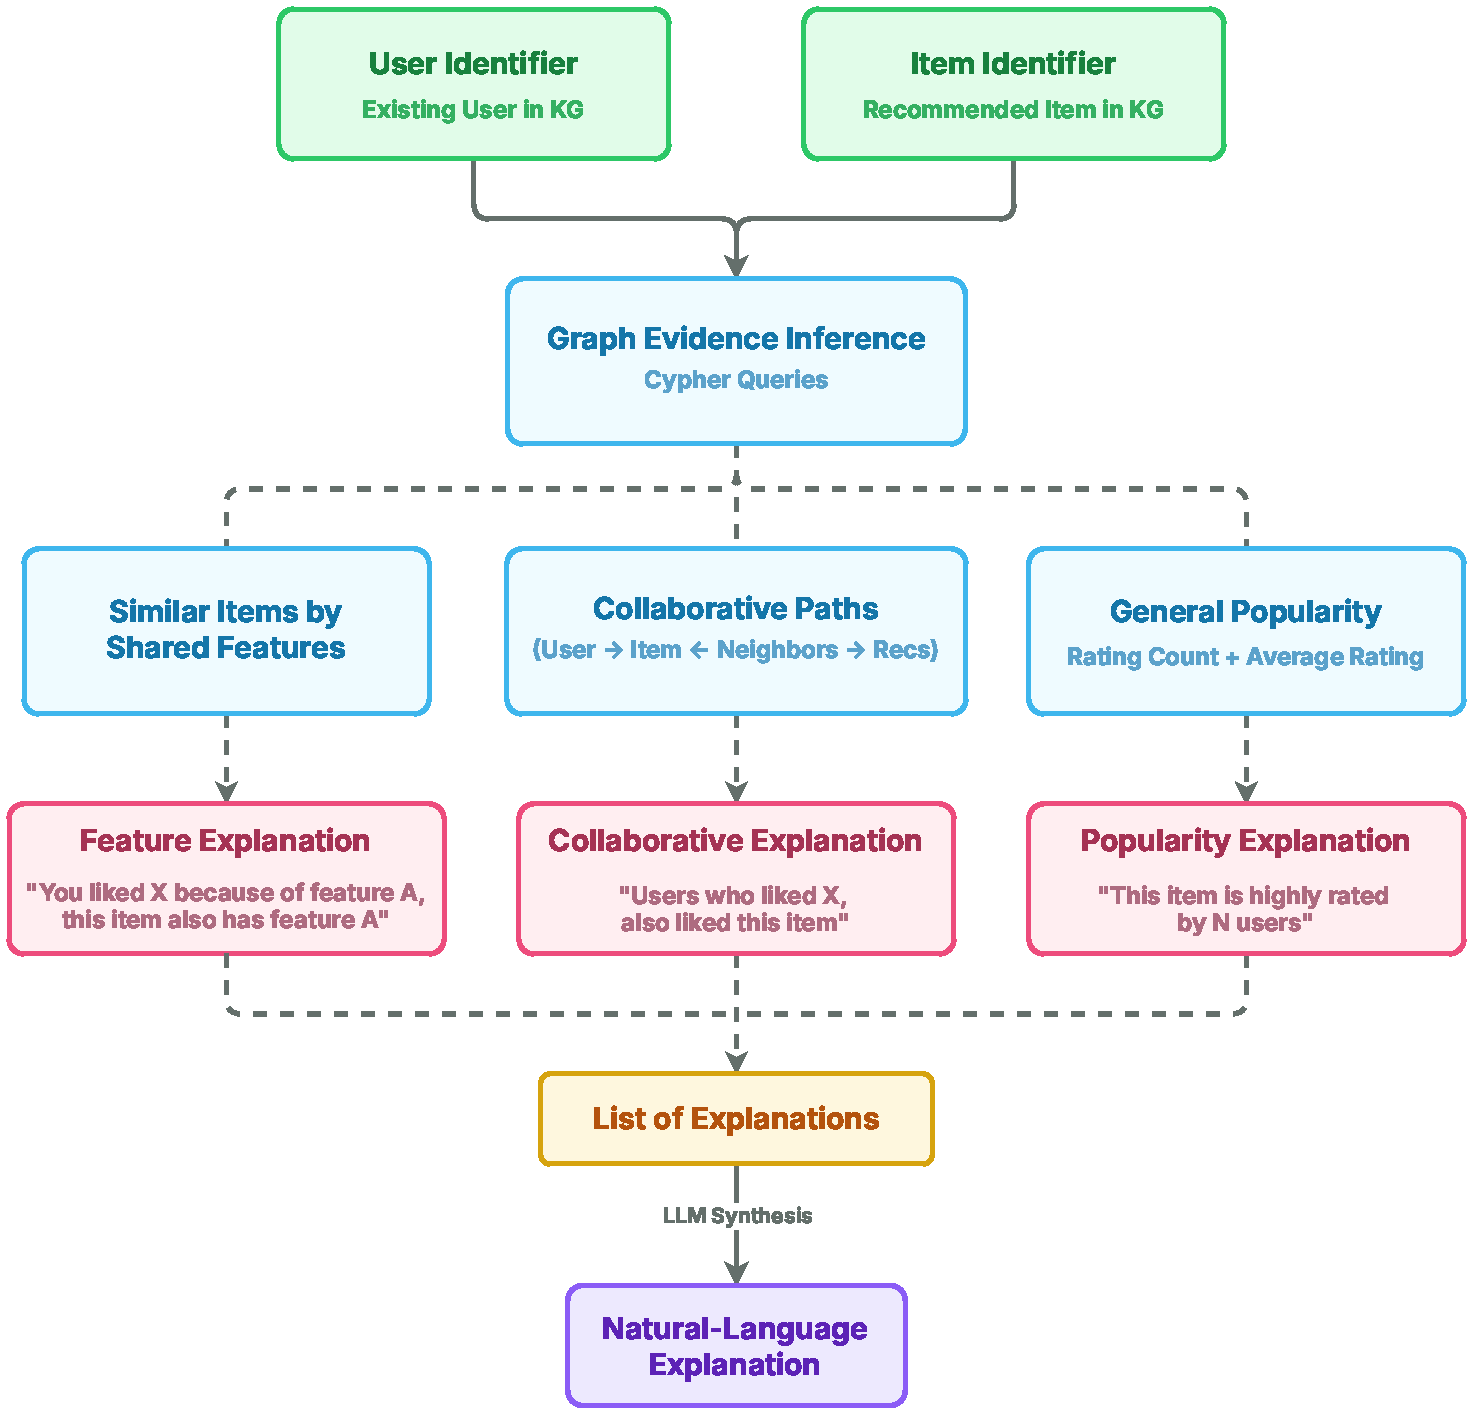
\includegraphics[width=\textwidth]{explanations.pdf}
\end{figure}